% L'option handout permet de supprimer la barre de navigation
\documentclass[handout]{beamer}
\usepackage[utf8]{inputenc}
\usepackage[english]{babel}
\usepackage[T1]{fontenc}
% Pour utiliser le signe €
\usepackage{eurosym}
% Pour pouvoir insérer des images
\usepackage{graphicx}
\usepackage{wrapfig}
\graphicspath{images/}
% Gestion des couleurs
\usepackage{color}
\definecolor{grey}{RGB}{0, 0, 0}

% Un joli thème flat
\usetheme{Rochester}

% Personnalisation du thème
\usecolortheme[named=grey]{structure}
% Numéro de slides dans le footer
\setbeamertemplate{footline}[frame number]
\setbeamertemplate{blocks}[shadow=false]

% ------------------------------------ %
% -- METADONNÉES DU DOCUMENT --------- %
\title{
	Teen Quotes
}
\author{
	Antoine \textsc{Augusti}
}
\date{}

\titlegraphic{\vspace{-30px}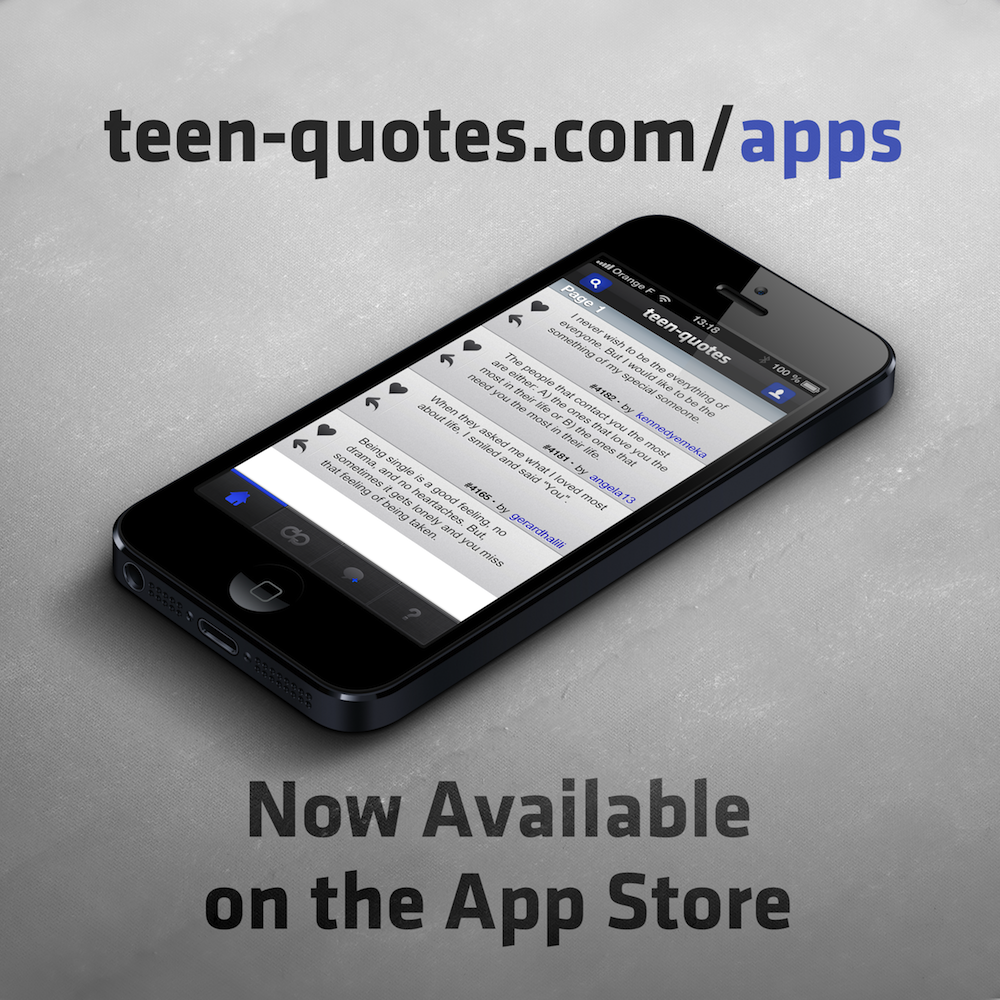
\includegraphics[width=60mm]{images/lancementTQ.png}}

% Début du document
\begin{document}
	
	% Génération de la page de titre
	\begin{frame}[plain]
		\titlepage
	\end{frame}

	% Génération du sommaire
	\begin{frame}[plain]
		\frametitle{Sommaire}
		\tableofcontents
	\end{frame}


	% ///////////////////////////////////// %
	% /// Teen Quotes today /////////////// %
	\section{Teen Quotes today}

	\subsection{What is Teen Quotes today}
	\begin{frame}
		\frametitle{What is Teen Quotes today}

		\begin{itemize}
			\item Simple goal: a single place on the Internet for teenagers who want to share their feelings.
			\item Headline: \textit{because some quotes are simply true}.
		\end{itemize}

		\begin{exampleblock}{Some numbers}
			2,2 M followers on Twitter, 1,7 M visitors on the website / mobile website / iOS application, 72 k followers on Instagram, 65 k likes on Facebook.
		\end{exampleblock}

	\end{frame}

	\subsection{Deep inside}
	\begin{frame}
		\frametitle{Deep inside}
		\begin{block}{Top 1 most favorited quote}
			``Boys think of girls just like books: if the cover doesn't catch their eyes, they won't even bother to read what's inside.''\\
			\#1716 - \textit{by mistichearts}
		\end{block}

		\begin{exampleblock}{Some more numbers}
			78 k tweets posted, 14 k quotes submitted (29 \% were accepted), 92 \% of our users are girls, 84 \% of our users are between 12 and 18 years old.
		\end{exampleblock}

	\end{frame}

	% /////////////////////////////////// %
	% /// How it started /////////////// %
	\section{How it started}
	
	\subsection{It's just a matter of luck... or almost}
	\begin{frame}
		\frametitle{It's just a matter of luck... or almost}

		\begin{itemize}
			\item It just started with a tweet: ``Please follow me, I've got something to tell you. It's a cool idea!''.
			\item Most of our users live in the USA, have got a smartphone... and use it a lot.
			\item The main goal was not to monetize, but everything is going well now.
		\end{itemize}

	\end{frame}

	% /////////////////////////////////// %
	% /// What I've learned /////////////// %
	\section{What I've learned}
	
	\subsection{An incredible and an ongoing experience}
	\begin{frame}
		\frametitle{An incredible and an ongoing experience}

		\begin{itemize}
			\item A technical challenge: to build a system that allows teenagers to share their fellings using a website, a mobile website or an iOS app.
			\item The feeling of being useful: teenagers relate to others. It helps them to live with their feelings.
			\item I (almost) read 14 000 quotes in 3 years because I moderate everything.
			\item I have improved my English ;-)
		\end{itemize}

	\end{frame}


% Fin du document
\end{document}